\documentclass[11pt]{article}
\pdfminorversion=7
\usepackage[utf8]{inputenc}
\usepackage[T1]{fontenc}
\usepackage[english]{babel}
\usepackage{lmodern,microtype}
\usepackage[a4paper,margin=25mm]{geometry}
\usepackage{amsmath,amssymb,bm,graphicx,booktabs,array,tabularx}
\usepackage[round,authoryear]{natbib}
\usepackage{enumitem,placeins,xcolor}
\usepackage[colorlinks=true,linkcolor=blue!45!black,citecolor=blue!45!black,urlcolor=blue!45!black]{hyperref}
\usepackage{caption,xurl}
\captionsetup{font=small,labelfont=bf}
\setlength{\parskip}{4pt}
\setlength{\parindent}{1em}
\setlength{\emergencystretch}{2em}
\setlength{\textfloatsep}{16pt}
\renewcommand{\topfraction}{0.9}
\renewcommand{\bottomfraction}{0.8}
\renewcommand{\textfraction}{0.08}
\renewcommand{\floatpagefraction}{0.45}
\setcounter{topnumber}{3}
\setcounter{totalnumber}{5}
\raggedbottom
\graphicspath{{figures/}}
\newcommand{\E}{\operatorname{E}}
\newcommand{\Var}{\operatorname{Var}}
\newcommand{\diag}{\operatorname{diag}}

\hypersetup{pdftitle={Bayesian spectral learning on road networks},pdfauthor={}}

\title{Bayesian spectral learning on road networks:	the role of topology, road attributes and segment length}
\author{}
\date{}
\begin{document}
\maketitle
\begin{abstract}
	Understanding spatial variation in network-constrained count data 
	requires statistical representations that account for network 
	topology, observed infrastructure characteristics, and the 
	definition of observational units. We proposed a Bayesian spectral 
	modelling framework for road-segment counts that combines a 
	negative-binomial likelihood with an eigenvalue-informed 
	continuous spike-and-slab prior. The framework quantifies 
	posterior evidence for individual network-derived spatial 
	patterns while retaining uncertainty in the complete spatial 
	field. Applications to road networks in Barcelona and Bogotá 
	demonstrate how the incorporation of road attributes and 
	alternative assumptions about segment length influence the 
	inferred spectral structure. Among 20 candidate spectral 
	components, expected posterior slab membership decreased from 
	6.92 to 1.31 in Barcelona and from 4.44 to 2.47 in Bogotá after 
	accounting for road attributes and estimating length elasticity. 
	Estimated elasticities were approximately 0.59 in both networks, 
	providing evidence against the assumption of proportionality 
	between expected counts and segment length. Despite reduced 
	slab membership, the spectral field improved pointwise 
	predictive performance relative to matched nonspatial models. 
	These findings highlight the distinction between spectral 
	component relevance and predictive spatial contribution, 
	providing a probabilistic framework for interpreting spatial 
	patterns in network-constrained geographical data. The graph-based 
	construction is transferable under its stated assumptions; the numerical 
	findings remain conditional on the two analysed networks.
\end{abstract}
\noindent\textbf{Keywords:}
Geographical information science;
network-constrained spatial data;
Bayesian spectral modelling;
spike-and-slab regularization;
road networks;
spatial count data.

\section{Introduction}
Counts observed along geographical networks raise a question about how spatial information is represented: should dependence be attached to intersections, road segments or Euclidean neighbourhoods, and what does a network-derived pattern mean once the observation model is specified? For segment counts, topology determines which observational units are connected, while recorded attributes and the assumed accumulation of counts with segment length affect the variation left for a spatial field. A spectral map therefore has two distinct interpretations: it can describe the chosen network representation, or it can describe a fitted contribution to the count process. Distinguishing them is a GIScience problem concerning the alignment of geographical representation, observational support and statistical inference.

Bayesian models have long been used for roadway counts and crash mapping \citep{song2006,aguerovalverde2008}. Intersection-based applications represent corridor dependence or interactions among closely spaced junctions \citep{guo2010,xie2014}, whereas segment and joint segment--intersection models recognize that the appropriate support depends on the response \citep{aguerovalverde2008,zenghuang2014}. If a segment response is explained by a latent intersection field, a node-to-edge projection is additionally required. Defining the field on segments avoids that projection, although segment support alone does not establish a new class of dependence.

Network representation is also a broader topic in geographical information modelling. For example, \citet{maduako2019} used a space-time varying graph to represent changing relationships among places and events. The present study concerns statistical inference on a fixed graph rather than dynamic graph representation or querying. Both involve the substantive choice of which geographical entities and relationships the representation preserves.

Eigenvector spatial filtering and graph signal processing already provide graph-adapted descriptions of spatial variation \citep{griffith2003,griffith2019,shuman2013}. Random-effects spectral models propagate coefficient uncertainty \citep{murakami2015}, and Bayesian dimension reduction and shrinkage address regularization and interactions with fixed effects \citep{hughes2013,donegan2020}. The random edge neighbourhood Gaussian model, RENeGe, supplies an existing segment-neighbourhood construction \citep{cruzreyes2023spasta}. The contribution here is therefore a specific inferential construction and interpretation on geographical edge support, rather than the introduction of spectral filtering or Bayesian shrinkage themselves.

We developed a negative-binomial model that combined shared-endpoint segment topology with an eigenvalue-informed continuous spike-and-slab prior. The ordered mixture scales support posterior allocation probabilities for individual candidate patterns, while all coefficient draws enter the spatial field and predictions. We distinguished the original operator eigenvectors, the centred and scaled regression columns, and the signed posterior contributions mapped on segments. We then kept the graph and candidate columns fixed within each network while changing the attribute and length specifications, so that changes in component evidence were attributable to the observation model rather than a different graph or basis.

\paragraph{Intellectual contribution to GIScience.}
The framework connects three objects that should not be interpreted interchangeably: the topology-derived candidate representation, posterior evidence about component allocation, and the geographical field entering prediction. It provides a model-based way to ask whether a mapped network pattern retains evidence after accounting for the attributes and support of the observational units. The induced covariance and limiting cases in Section~\ref{sec:induced_covariance} explain why weak slab membership does not imply an absent spatial field: a continuous spike retains nonzero prior variation on the chosen graph-derived subspace. The contribution is the joint treatment of geographical support, component-specific uncertainty and predictive use of that representation. It is not a claim of an exact reduction of the full RENeGe covariance or universal improvement over other shrinkage methods.

\paragraph{Scope of generalization.}
The mathematical construction does not require Barcelona- or Bogot\'a-specific coordinates, road categories or response values. It applies to a finite undirected segment-neighbourhood graph with positive degrees, nonconstant retained columns, and a positive length or exposure measure, when a negative-binomial observation model and the stated log-linear mean are appropriate. With $0\leq\gamma<1$, normalized-adjacency eigenvalues in $[-1,1]$ give positive variance denominators; the induced covariance and the continuous-spike limiting behaviour follow for any such fixed basis. These are transferable properties of the formulation. Application to a new network requires reconstructing its adjacency and basis, choosing its candidate dimension, defining suitable attributes and exposure, and refitting and checking the model; it does not transfer the fitted coefficients or component identities between cities. Directed flow, temporal dynamics, disconnected or isolated units and alternative segmentation require separate treatment or validation.

The empirical analyses have a narrower scope. We investigated source-record counts in two urban networks to illustrate the framework under different geographical configurations. The two cases were not a probability sample of cities or a spatial-transfer experiment. Neither a length elasticity near 0.59, a decrease in expected slab membership, nor a predictive gain is asserted to hold on every road network. Their direction and magnitude depend on data provenance, network representation, available attributes, the observation model and the candidate basis. The general contribution is the reusable construction and the separation of inferential objects; cross-network performance and substantive crash relationships remain empirical questions.

Specifically, the study addressed three questions:
\begin{enumerate}
\item How can an edge-supported model distinguish topology-derived patterns, posterior component allocation and geographical contributions to a network count field?
\item In the two applications, how did adjustment for recorded road attributes and estimation of length elasticity change evidence for the same candidate patterns?
\item Within matched specifications, did continuous spectral regularization retain predictive spatial information when component allocation became weaker?
\end{enumerate}

For readers analysing other network-supported counts, the resulting workflow offers a way to separate a structural property of the GIS representation from evidence supplied by a fitted observation model. It also provides a reporting rule: component membership, signed field maps, predictive scores and adequacy checks should be reported as complementary quantities. Potential extensions to infrastructure-failure or other segment-count processes require domain-appropriate observation and exposure definitions and fresh validation; they were not evaluated in the present applications.

\section{Road networks, counts and recorded attributes}
\subsection{Observational support and analytical samples}
The analyses used frozen municipal source records and road-network snapshots with OpenStreetMap-derived attributes. We reconstructed the segment counts from the source rows using the archived spatial assignment rules before fitting the models. We reconstructed binary segment adjacency from shared endpoints, retained the connected component containing the greatest number of segments, and preserved the original segment order. Parallel road features were retained; a pair sharing both endpoints received one binary adjacency entry. Independent reconstruction of the adjacency directly from the retained geometries reproduced the matrix used in the models. The reconstructed responses and every model input matched the archived inputs exactly; this verifies computational provenance while preserving the original counting and assignment rules.

The Barcelona source contains 2,714 segments. Its retained component has 2,540 segments and 2,028 intersections. The Bogot\'a source contains 8,169 segments; its retained component has 6,079 segments and 5,107 intersections. Component restriction excludes 174 and 2,090 segments, respectively. The resulting inference is conditional on the retained networks. Characteristics of excluded components and sensitivity to the study boundary have not been evaluated. Table~\ref{tab:data} describes only the retained analytical support.

\begin{table}[tb]
\centering\small
\caption{Retained analytical samples. Totals count source records: accident-report rows in Barcelona and person-involvement rows in Bogot\'a. They are not directly comparable counts of distinct crashes.}
\label{tab:data}
\begin{tabular}{lrr}\toprule
Characteristic & Barcelona & Bogot\'a\\\midrule
Retained segments & 2,540 & 6,079 \\
Retained intersections & 2,028 & 5,107 \\
Recovered total count &  3,735 & 85,068 \\
Represented length (km) & 224.9 & 779.0 \\
Zero-count segments (\%) & 54.0 & 28.3 \\
\bottomrule
\end{tabular}
\end{table}

\subsection{Response recovery and provenance}
We reconstructed Barcelona counts from the 2023 Guardia Urbana accident-report file (7,724 rows and 7,721 distinct incident identifiers). We retained repeated report rows, transformed coordinates to EPSG:25831, restricted records to the frozen road snapshot bounding box and assigned each remaining row to its nearest road feature. We reconstructed Bogot\'a counts from the frozen person-involvement source file covering 2007--2025 (468,551 rows and 324,962 distinct incident identifiers). We transformed coordinates to EPSG:3116, retained valid rows within the full road snapshot bounding box, assigned them to the nearest feature in that snapshot, aggregated by OpenStreetMap identifier and inherited those counts on the selected road features. Thus, multiple people involved in one crash contributed multiple records in Bogot\'a. Neither response was deduplicated into distinct crashes.

The source reconstruction reproduced every archived segment count and all inputs to the 20 fitted specifications exactly. After restricting to the greatest connected component, the totals were 3,735 report rows in Barcelona and 85,068 person-involvement rows in Bogot\'a. The original aggregation in Bogot\'a preceded clipping the selected road geometries, so counts on an inherited OpenStreetMap feature can include contributions from its clipped-away portions. The archived support and this assignment rule were preserved to reproduce the reported analysis; they do not define incidence strictly within the final clipped geometry. Source hashes, coordinate exclusions, assignments and distances are exported by the shared workflow. The two responses describe different record units and observation periods; their magnitudes are not comparable estimates of city-wide crash incidence. All numerical results refer to the retained 2,540-segment and 6,079-segment networks.

Segment lengths were recomputed from the projected geometries: ETRS89/UTM zone 31N for Barcelona and EPSG:3116 for Bogot\'a. Length measures the amount of represented roadway, not vehicle flow. No traffic-volume-adjusted risk is estimated, and different observation periods prevent substantive cross-city comparisons of count levels.

\subsection{Covariate construction}
The common road attributes are road class, lane-count category and surface tag. Road class is recorded for all retained features and has four categories: residential, tertiary, secondary and primary. Residential roads form the reference group. Lane counts are grouped as one, two, three or more, and unknown, with two lanes as reference. A recorded value of 22 in Bogot\'a was flagged as implausible for this analysis and assigned to the unknown category. Unknown lane counts occur on 430 Barcelona segments (16.9\%) and 498 Bogot\'a segments (8.2\%).

Surface tags are grouped as \texttt{asphalt}, another recorded tag, and unknown. Another tag includes generic \texttt{paved} as well as more specific materials; it cannot be interpreted uniformly as absence of asphalt. Only 22 Barcelona segments have another recorded surface tag, compared with 583 in Bogot\'a. Surface is unknown on 138 and 160 segments. Unknown categories are nuisance controls for recording patterns, not observations that the corresponding infrastructure is absent. Complete category counts and coefficient summaries are supplied in the supplementary material.

The attributes have not been harmonized historically with the crash observation periods. Their coefficients are conditional associations within these prepared datasets, not historical causal effects. We avoided selecting additional covariates from incomplete speed or width fields at this stage. Road attributes are introduced as a fixed, interpretable set; they are not selected by the spectral mixture.

\section{A segment-supported spectral representation}
\subsection{From road topology to candidate patterns}
Let $G=(V,E)$ be an undirected road graph and let $n=|E|$ denote the number of retained segments. Define the $n\times n$ binary matrix $A$ by $A_{er}=1$ when distinct segments $e$ and $r$ share an endpoint. Its diagonal is zero. This is a simple edge-neighbourhood, or line-graph, representation of the road network. With $D=\diag(A\bm 1)$, define the symmetric normalized adjacency
\begin{equation}
 S=D^{-1/2}AD^{-1/2}=U\Delta U^{\mathsf T},
 \qquad \Delta=\diag(\delta_1,\ldots,\delta_n).
 \label{eq:operator}
\end{equation}
Eigenvalues lie in $[-1,1]$ and are ordered decreasingly. For a connected retained component, $\delta_1=1$ and the Perron eigenvector is proportional to $D^{1/2}\bm 1$. It is generally not constant. The normalized Laplacian $I-S$ has eigenvalues $1-\delta_j$, so leading adjacency eigenvectors encode low graph-frequency patterns in this normalized representation. The ordering concerns the source eigenvectors and does not assign a physical distance scale to each mode.

We computed the leading 61 eigenpairs for descriptive examination. The largest eigen-equation residual norm was below $6\times10^{-11}$ in both networks. For model fitting, the candidate set is $u_2,\ldots,u_{21}$, with $M=20$ and $\lambda_j=\delta_{j+1}$. All reported candidate indices start at one after omission of Perron. Figure~\ref{fig:spectrum} shows the upper end of the spectrum; Figure~\ref{fig:raw} maps the first three candidate eigenvectors. Only the upper spectrum was computed, so these figures do not describe the full range of network frequencies or justify a global variance-explained claim.

\begin{figure}[tb]\centering
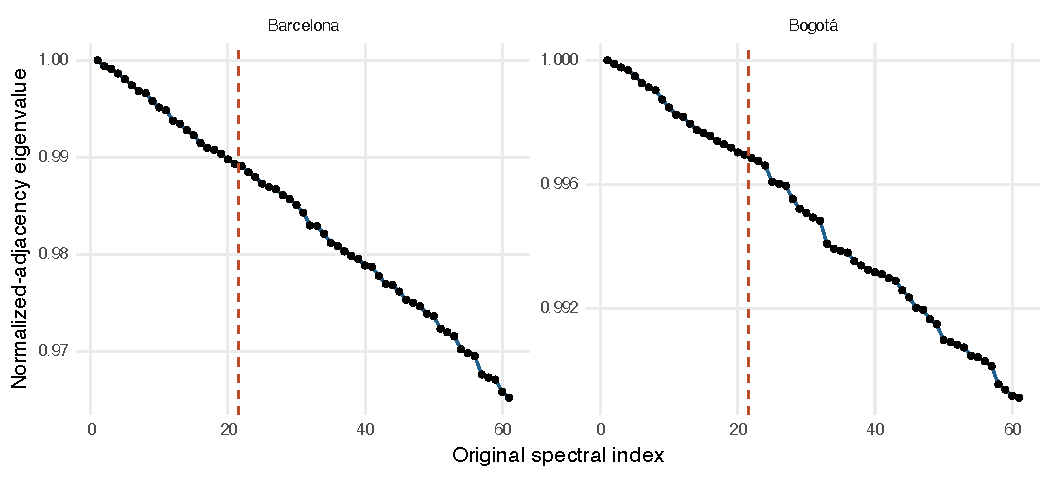
\includegraphics[width=\textwidth]{spectrum.pdf}
\caption{Leading normalized-adjacency eigenvalues. Original index 1 is Perron; indices 2--21 enter the candidate set. The dashed boundary separates fitted candidates from additional eigenpairs computed for description. Vertical scales differ between cities.}
\label{fig:spectrum}\end{figure}
\begin{figure}[p]\centering
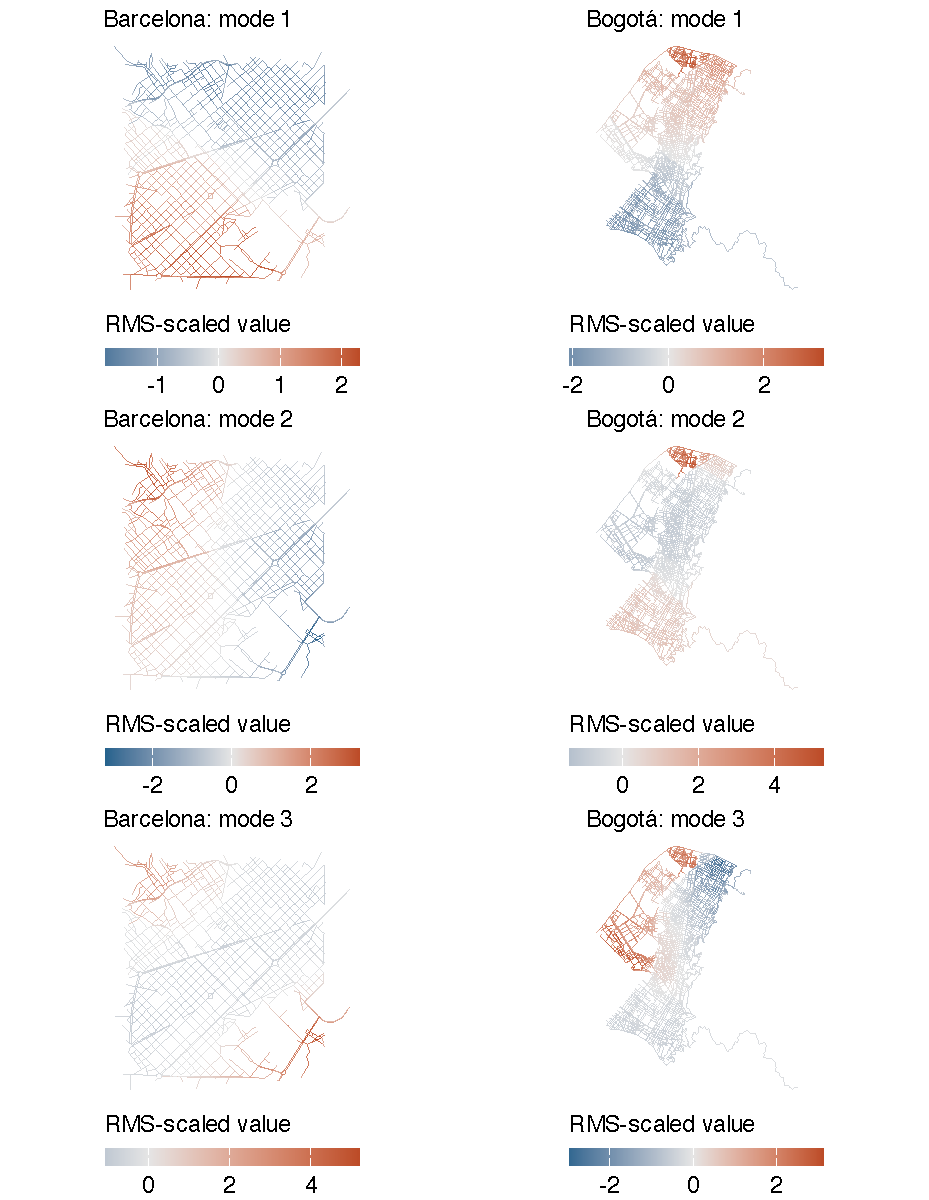
\includegraphics[width=\textwidth]{raw_network_modes.pdf}
\caption{First three candidate eigenvectors in each retained network, scaled to unit root-mean-square without centering. Scalar rescaling preserves their eigenvector property. Signs are arbitrary, and colours represent graph contrasts rather than estimated crash effects. Each panel has its own legend.}
\label{fig:raw}\end{figure}

\subsection{Regression columns and the RENeGe connection}
For $v_j=u_{j+1}$, the fitted column is
\begin{equation}
 B_{ej}=\frac{v_{ej}-\bar v_j}{\{n^{-1}\sum_{r=1}^n(v_{rj}-\bar v_j)^2\}^{1/2}},
 \qquad \bar v_j=n^{-1}\sum_{e=1}^n v_{ej}.
 \label{eq:basis}
\end{equation}
Centering removes the intercept direction and RMS scaling puts coefficient scales on a comparable footing. These operations do not generally preserve mutual orthogonality or the eigenvector property. The fitted field $s=Bb$ is therefore expressed in graph-derived columns whose source ordering is spectral, rather than in an unchanged orthonormal eigenbasis.

The eigenvalue weighting is motivated by the proper edge-neighbourhood precision $Q(\gamma)=\kappa(D-\gamma A)$ \citep{cruzreyes2023spasta}. Its exact covariance is
\begin{equation}
 Q(\gamma)^{-1}=\kappa^{-1}D^{-1/2}U
 \diag\{(1-\gamma\delta_j)^{-1}\}U^{\mathsf T}D^{-1/2}.
\end{equation}
Our regression uses the transformed $B$ and omits the external degree factors. It is an operator-inspired low-rank construction, not an exact reparameterization of this full Gaussian field. Omitting Perron is likewise a modelling restriction: since Perron is degree-related before transformation, omission can remove more than an intercept. These distinctions are important for interpreting what the candidate set can represent.

Eigenvector signs are arbitrary. Consequently, interpretation uses a signed posterior contribution $a_j=B_j\E(b_j\mid Y)$, which is invariant to simultaneously reversing a column and its coefficient. We ranked posterior mean contributions by their RMS magnitudes and mapped the signed contributions themselves. This differs from interpreting an unweighted eigenvector as an estimated crash pattern.

\FloatBarrier
\section{Bayesian count model and comparison design}
\subsection{Road attributes and the length assumption}
For segment $e$, let $L_e$ be length in kilometres and $x_e$ the eight indicator variables formed from the recorded road attributes. We used the negative-binomial parameterization
\begin{align}
 Y_e\mid\mu_e,\phi&\sim\operatorname{NegBinomial}_2(\mu_e,\phi),\\
 \log\mu_e&=\log L_e+\alpha+x_e^{\mathsf T}\beta
      +d\{\log L_e-\overline{\log L}\}+s_e,
 \label{eq:count}
\end{align}
where $\Var(Y_e\mid\mu_e,\phi)=\mu_e+\mu_e^2/\phi$. The primary comparison sets $d=0$, imposing proportional accumulation of expected counts with length. The sensitivity analysis estimates $d$, giving the total length elasticity $\ell=1+d$. Centering changes the intercept interpretation, not the elasticity. When $\ell$ is estimated, the target is an expected count conditional on length and recorded attributes; it should not be described as a constant frequency per kilometre.

We assigned $\alpha\sim N(0,5^2)$, each recorded-attribute coefficient $\beta_k\sim N(0,0.7^2)$ and $\phi\sim\operatorname{Exponential}(0.5)$, with the exponential expressed by its rate. In the estimated-length analysis $d\sim N(0,0.7^2)$, so $\ell\sim N(1,0.7^2)$. These priors are independent of the full-data empirical mean. Unknown-category coefficients receive the same regularization as other indicators but are not given physical interpretations.

\subsection{Ordered continuous spike-and-slab regularization}
The spatial field in the mixture spectral model is $s=Bb$. For $j=1,\ldots,M$, define latent membership $z_j$ and
\begin{align}
 z_j\mid\pi&\sim\operatorname{Bernoulli}(\pi), & \pi&\sim\operatorname{Beta}(1,4),\\
 b_j\mid z_j=0&\sim N(0,\sigma_0^2), & \sigma_0&=0.05,\\
 b_j\mid z_j=1,\tau&\sim N(0,\sigma_{1j}^2), &
 \sigma_{1j}^2&=\sigma_0^2+\frac{\tau^2}{1-\gamma\lambda_j},\\
 \tau&\sim N^+(0,0.5^2), & \gamma&=0.9.
 \label{eq:mixture}
\end{align}
The additive spike variance ensures an ordered wider component for $\tau>0$. Larger source eigenvalues permit greater slab variance. The resulting prior shrinks coefficients continuously; it does not set them exactly to zero. Membership probabilities
\begin{equation}
 p_j=\Pr(z_j=1\mid Y)
 =\E\left[\frac{\pi f_N(b_j;0,\sigma_{1j}^2)}
 {\pi f_N(b_j;0,\sigma_{1j}^2)+(1-\pi)f_N(b_j;0,\sigma_0^2)}\;\middle|\;Y\right]
\end{equation}
are recovered after integrating the binary indicators out of the sampling target. They measure posterior allocation to the slab, not the probability that a coefficient is nonzero. When the component scales are close, membership is intrinsically less differentiated.

For $K=\sum_jz_j$, $\E(K\mid Y)=\sum_jp_j$. We also computed its posterior distribution by averaging conditional Poisson-binomial distributions across draws. Quantiles of $K$ are therefore distinct from quantiles of the draw-wise sum of conditional membership probabilities. A threshold of 0.5 is used only to summarize membership descriptively. All coefficient draws contribute to posterior fields and predictions, including coefficients allocated predominantly to the continuous spike. Neither $\E(K\mid Y)$ nor the number above 0.5 is a literal rank of the fitted field.

\subsection{Induced covariance and properties of the spectral field}
\label{sec:induced_covariance}

The proposed hierarchical prior induces a structured covariance 
on the geographical support of the road network. Let

\begin{equation}
	\mathbf{s} = \mathbf{B}\mathbf{b},
\end{equation}

where $\mathbf{B}\in\mathbb{R}^{n\times M}$ contains the 
transformed graph-derived spectral columns and
$\mathbf{b}=(b_1,\ldots,b_M)^\top$ denotes the corresponding 
regression coefficients.

Conditional on the membership indicators $\mathbf{z}$ and 
the global slab scale $\tau$, the coefficients satisfy

\begin{equation}
	b_j \mid z_j,\tau
	\sim
	\mathcal{N}\left(
	0,
	\sigma_0^2+
	z_j\frac{\tau^2}{1-\gamma\lambda_j}
	\right).
\end{equation}

Define

\begin{equation}
	\mathbf{V}_{\mathbf{z}}
	=
	\operatorname{diag}\left(
	\sigma_0^2+
	z_j\frac{\tau^2}{1-\gamma\lambda_j}
	\right)_{j=1}^{M}.
\end{equation}

Under conditional independence of the spectral coefficients,
the induced conditional distribution of the spatial field is

\begin{equation}
	\mathbf{s}\mid\mathbf{z},\tau
	\sim
	\mathcal{N}_n\left(
	\mathbf{0},
	\mathbf{B}\mathbf{V}_{\mathbf{z}}\mathbf{B}^{\top}
	\right),
\end{equation}

where the Gaussian distribution may be degenerate because 
the covariance matrix has rank at most $M$.

Integrating over the membership indicators, with
$z_j\mid\pi\sim\operatorname{Bernoulli}(\pi)$, yields

\begin{equation}
	\mathbb{E}(\mathbf{s}\mid\pi,\tau)
	=
	\mathbf{0},
\end{equation}

and

\begin{equation}
	\operatorname{Cov}(\mathbf{s}\mid\pi,\tau)
	=
	\mathbf{B}
	\operatorname{diag}\left(
	\sigma_0^2+
	\frac{\pi\tau^2}{1-\gamma\lambda_j}
	\right)_{j=1}^{M}
	\mathbf{B}^{\top}.
	\label{eq:induced_covariance}
\end{equation}

The marginal distribution obtained by integrating over
$\mathbf{z}$ is generally a Gaussian mixture rather than
a single Gaussian distribution.

In particular, the induced prior covariance between two road 
segments $e$ and $r$ is

\begin{equation}
	\operatorname{Cov}(s_e,s_r\mid\pi,\tau)
	=
	\sum_{j=1}^{M}
	B_{ej}B_{rj}
	\left(
	\sigma_0^2+
	\frac{\pi\tau^2}{1-\gamma\lambda_j}
	\right).
	\label{eq:segment_covariance}
\end{equation}

Equation~\eqref{eq:segment_covariance} illustrates how 
network-derived spatial patterns determine the dependence 
between road segments. Dependence is represented through 
shared spectral structure rather than being specified directly 
as a function of Euclidean distance.

For $\gamma>0$, the eigenvalue-informed variance component 
satisfies

\begin{equation}
	\frac{\partial}{\partial\lambda_j}
	\left(
	\frac{\tau^2}{1-\gamma\lambda_j}
	\right)
	=
	\frac{\gamma\tau^2}
	{(1-\gamma\lambda_j)^2}
	>0,
\end{equation}

for $\tau>0$. Consequently, spectral components associated 
with larger eigenvalues receive greater prior slab variance, 
allowing broader variation along the corresponding 
low-frequency network patterns.

The strength of this differential regularization depends on 
both $\gamma$ and the dispersion of the retained eigenvalues.
When the candidate eigenvalues are closely concentrated, 
the eigenvalue-informed slab approaches an approximately 
homogeneous variance specification.

\subsection{Nonspatial, dense spectral and BYM2-type comparisons}
The nonspatial model sets $s=0$. The dense spectral comparator has $b_j=\tau w_j\xi_j$, where $w_j=(1-\gamma\lambda_j)^{-1/2}$, $\xi_j\sim N(0,1)$ and $\tau\sim N^+(0,0.5^2)$. It retains the complete candidate set without mixture membership. Its label denotes the common low-rank operator-derived representation, not a fitted full-rank CAR model.

The BYM2-type comparator combines a scaled structured field and independent segment effects, following the scaling rationale of \citet{riebler2016}. Let $R=B\diag(w_j)$ and
\begin{equation}
 c^2=\exp\left\{\frac{1}{n}\sum_e\log[(RR^{\mathsf T})_{ee}]\right\}.
\end{equation}
With independent standard normal vectors $\xi$ and $v$, its field is
\begin{equation}
 s=\sigma\{\sqrt{\rho}\,R\xi/c+\sqrt{1-\rho}\,v\},\qquad
 \sigma\sim N^+(0,0.5^2),\quad\rho\sim\operatorname{Beta}(0.5,0.5).
\end{equation}
The structured component has unit geometric-mean marginal variance before multiplication by its scale. This is a spectral BYM2-type comparator on the retained basis, not a full-rank BYM2 analysis.

The primary experiment contains four model families, two cities and two attribute specifications: unadjusted (U) and road-attribute adjusted (C), both imposing $\ell=1$. Four additional fits estimate length (L): nonspatial and mixture spectral models in both cities, with the same recorded attributes. This gives 20 fitted specifications. Dense spectral and BYM2-type models with estimated length were not fitted, so the additional L comparison is matched only between nonspatial and mixture spectral models.


\paragraph{Limiting behaviour.}

The induced covariance provides a unified interpretation 
of several limiting cases of the proposed formulation.

First, when $\pi\rightarrow 0$,

\begin{equation}
	\operatorname{Cov}(\mathbf{s}\mid\pi,\tau)
	\longrightarrow
	\sigma_0^2\mathbf{B}\mathbf{B}^{\top}.
\end{equation}

The spatial field remains continuously regularized rather 
than being constrained to zero.

Second, when $\pi\rightarrow 1$,

\begin{equation}
	\operatorname{Cov}(\mathbf{s}\mid\pi,\tau)
	\longrightarrow
	\mathbf{B}
	\operatorname{diag}\left(
	\sigma_0^2+
	\frac{\tau^2}{1-\gamma\lambda_j}
	\right)_{j=1}^{M}
	\mathbf{B}^{\top}.
\end{equation}

This corresponds to allocation of all candidate components 
to the wider mixture distribution.

Under the additional limit $\sigma_0\rightarrow 0$, the 
resulting covariance becomes

\begin{equation}
	\tau^2\mathbf{B}
	\operatorname{diag}\left(
	\frac{1}{1-\gamma\lambda_j}
	\right)_{j=1}^{M}
	\mathbf{B}^{\top},
\end{equation}

recovering the covariance structure of the dense spectral 
comparator considered in this study.

Finally, setting $\gamma=0$ removes eigenvalue-dependent 
differentiation between slab variances. The prior then reduces 
to a continuous spike-and-slab specification with a common 
slab variance across the retained spectral components.

These relationships clarify how the proposed formulation 
connects continuous spectral shrinkage, dense spectral 
regularization, and conventional mixture-based priors 
within a common edge-supported representation.


\subsection{Computation, prediction and adequacy}
All models were sampled in CmdStan 2.36.0 using four chains. Initial runs used 1,000 warm-up and 1,000 retained iterations per chain, target acceptance 0.99 and maximum tree depth 13. A diagnostic-triggered rerun used 2,000 warm-up and 2,000 retained iterations, target acceptance 0.995 and depth 14. The operational pass criterion required no divergences or depth saturation, maximum rank-normalized $\widehat R\leq1.01$, minimum bulk effective sample size of 400 and minimum chain E-BFMI of 0.3. We monitored mixture probabilities as well as core parameters; BYM2-type fits also included checks of independent effects. Rank and effective-size diagnostics follow the principles described by \citet{vehtari2021}.

Pointwise Pareto-smoothed importance-sampling leave-one-out evaluation uses up to 2,000 evenly spaced posterior draws and relative-efficiency adjustment \citep{vehtari2017}. For BYM2-type prediction, the held-out independent segment effect is integrated against its normal prior, rather than evaluated using that segment's fitted effect. Normal quadrature starts with 30 nodes and is checked against 60 on high-count and control segments; all segment likelihoods are recomputed with 60 nodes if the maximum checked log-density discrepancy exceeds 0.001. The paired standard error of an ELPD difference is computed from its segment-wise differences.

This procedure leaves neighbouring observations available to the shared spatial field. It evaluates interpolation-like prediction on the retained network, not transfer to unseen districts. Segment-wise standard errors do not replace a spatially blocked experiment. Pareto diagnostics are reported alongside scores, and influential observations require exact refits or an alternative validation design before a definitive ranking.

Posterior predictive checks use 400 replicated datasets to examine the mean, variance, zero fraction, maximum and 99th percentile. A further check compares Moran's $I$ for centred Pearson residuals on the segment graph using 100 posterior draws. These are conditional adequacy checks; they address different questions from sampling convergence or out-of-sample scoring. Field maps use posterior means and marginal 90\% intervals, without simultaneous multiplicity adjustment.

\section{Results}
\subsection{Adjustment changes component membership}
Figure~\ref{fig:membership} shows how posterior membership changes while the graph and candidate set remain fixed. In Barcelona, expected slab membership falls from 6.92 under U to 2.27 under C and 1.31 under L. Modes 1, 2, 8 and 15 exceed 0.5 under U; none does after attribute adjustment. Under L, the largest membership probability is only 0.16. This indicates weak allocation to the wider mixture component, not that every spatial coefficient is zero.

In Bogot\'a, expected membership falls from 4.44 to 2.89 and then 2.47. Modes 1, 6 and 14 exceed 0.5 under U. After attribute adjustment, modes 1 and 6 remain above that descriptive threshold, at approximately 0.67 and 0.61. Under L, mode 1 has probability 0.56 and mode 6 decreases to 0.39. The surviving allocation is moderate rather than decisive. The posterior distributions of $K$ are broad (Table~\ref{tab:membership}); point estimates alone would overstate certainty about a compact set.

\begin{figure}[p]\centering
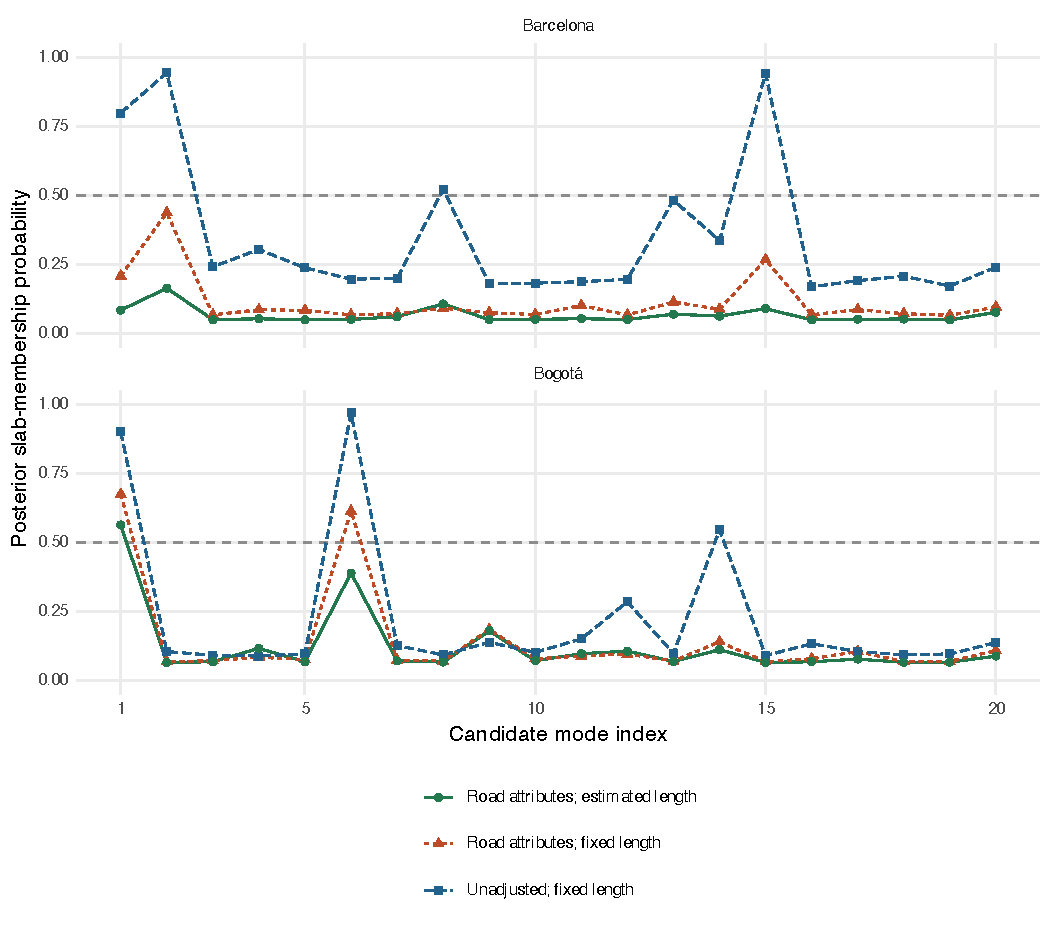
\includegraphics[width=\textwidth]{mode_membership.pdf}
\caption{Posterior slab-membership probabilities for the same 20 candidate columns within each city. U: unadjusted, fixed unit length coefficient; C: recorded road attributes, fixed length coefficient; L: recorded attributes and estimated length coefficient. The dashed 0.5 line is descriptive and is not used to truncate predictions.}
\label{fig:membership}\end{figure}
\begin{table}[tb]\centering\small
\caption{Posterior mixture membership. Intervals refer to the latent membership count $K$, not to an exact number of nonzero regression coefficients. U, C and L are defined in Figure~\ref{fig:membership}.}
\label{tab:membership}
\begin{tabular}{llrcl}\toprule
Network & Specification & $\E(K\mid Y)$ & 90\% interval for $K$ & Modes with $p_j>0.5$\\\midrule
Barcelona & U & 6.92 & [2, 13] & 1, 2, 8, 15 \\
Barcelona & C & 2.27 & [0, 8] & None \\
Barcelona & L & 1.31 & [0, 7] & None \\
Bogotá & U & 4.44 & [1, 9] & 1, 6, 14 \\
Bogotá & C & 2.89 & [0, 8] & 1, 6 \\
Bogotá & L & 2.47 & [0, 8] & 1 \\
\bottomrule
\end{tabular}\end{table}

\FloatBarrier
\subsection{Length sensitivity and recorded road attributes}
In the mixture spectral L model, length elasticities are 0.585 (90\% interval 0.533--0.638) in Barcelona and 0.590 (0.561--0.617) in Bogot\'a. Matched nonspatial estimates are 0.584 (0.531--0.638) and 0.596 (0.567--0.624). Within these specifications, the posterior intervals are well below the imposed unit coefficient. This is evidence against that proportionality assumption in the prepared data, not an estimate of the causal effect of extending a road.

Allowing length to be estimated improves the mixture model's ELPD by 76.3 (paired SE 17.1) in Barcelona and 265.3 (30.3) in Bogot\'a relative to C. The corresponding nonspatial gains are 76.8 (18.5) and 252.3 (29.4). The agreement across spatial and nonspatial fits indicates that the sensitivity is not confined to a particular spatial prior. Differences in traffic volume, segmentation and road function may all contribute to the subproportional association; the available variables cannot separate them.

Table~\ref{tab:effects} reports conditional count ratios from the mixture L models. Comparisons hold recorded attributes and length fixed. They describe associations with the recorded categories; surface-tag comparisons in Barcelona are particularly limited by the small number of alternative recorded tags. Coefficients for unknown categories are retained in estimation and supplied separately, rather than interpreted as infrastructure effects.

\begin{table}[tb]\centering\small
\caption{Conditional count ratios from the mixture spectral model with recorded attributes and estimated length. Values are posterior medians with marginal 90\% intervals. The table excludes nuisance coefficients for unknown categories.}
\label{tab:effects}
\begin{tabular}{p{.42\textwidth}rr}\toprule
Recorded category comparison & Barcelona & Bogot\'a\\\midrule
Tertiary vs residential road & 1.14 [0.95, 1.35] & 1.95 [1.78, 2.13] \\
Secondary vs residential road & 0.97 [0.80, 1.18] & 2.59 [2.36, 2.84] \\
Primary vs residential road & 1.29 [1.04, 1.60] & 3.73 [3.35, 4.17] \\
One vs two lanes & 0.84 [0.69, 1.03] & 1.07 [0.95, 1.20] \\
Three or more vs two lanes & 1.49 [1.27, 1.74] & 1.29 [1.17, 1.43] \\
Other surface tag vs asphalt & 0.86 [0.52, 1.48] & 0.82 [0.73, 0.92] \\
\bottomrule
\end{tabular}\end{table}

\subsection{Signed spatial contributions and uncertainty}
Figure~\ref{fig:contributions} displays the three largest posterior mean contributions by RMS in each L fit. Their ranking differs from ranking membership probabilities: a column can contribute to the field even when its coefficient is predominantly allocated to the continuous spike. The maps display signed combinations of column and coefficient, so their interpretation is unaffected by an arbitrary eigenvector sign reversal. These contributions are conditional log-count contrasts, not traffic-adjusted risk surfaces.

The complete posterior mean fields (Figure~\ref{fig:field}) combine all 20 coefficients. They should not be reconstructed by retaining only the modes above 0.5. Marginal interval maps in the supplementary material identify segments whose field intervals contain zero and distinguish that uncertainty from mixture membership. Such segment-wise intervals do not establish jointly significant hotspot regions. Neither road class nor length adjustment yields a causal decomposition between infrastructure and spatial effects, and collinearity between attributes and graph-derived columns remains possible.

\begin{figure}[p]\centering
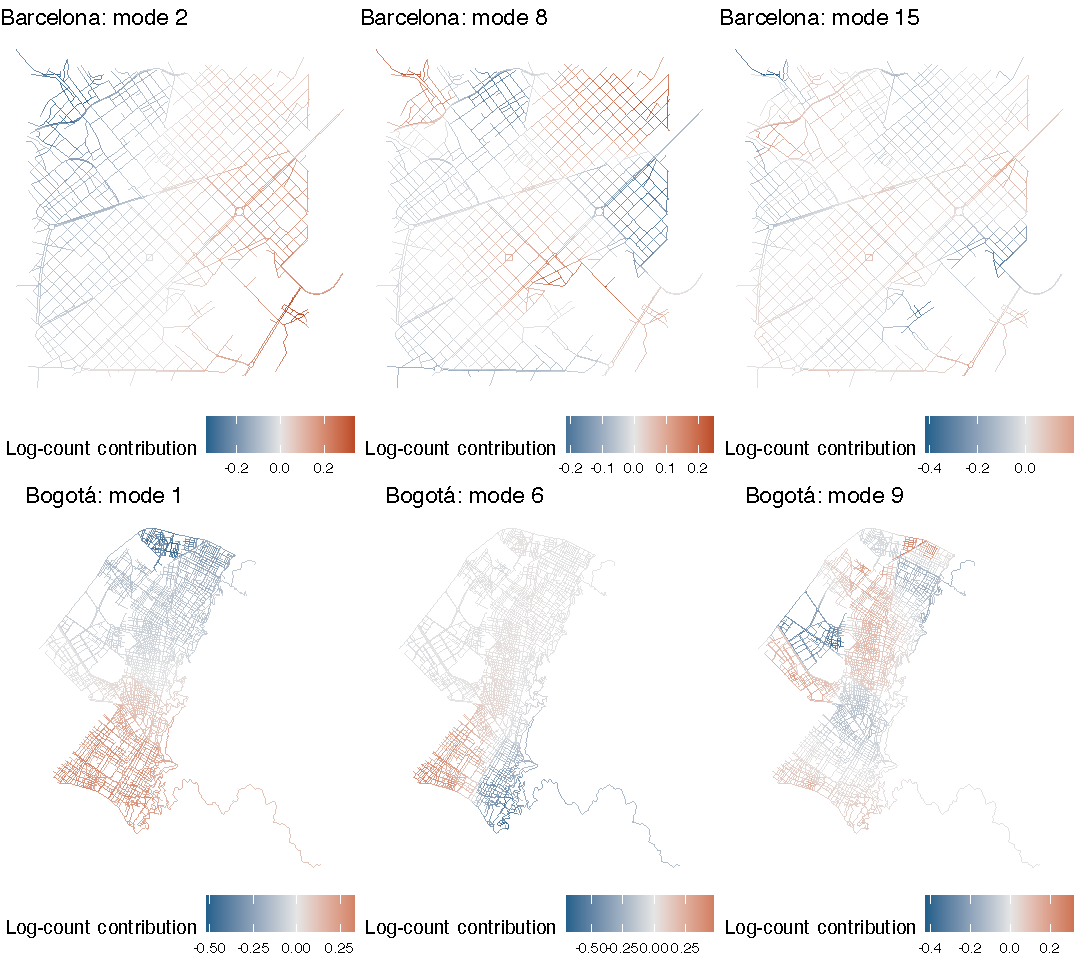
\includegraphics[width=\textwidth]{adjusted_contributions.pdf}
\caption{Three largest RMS posterior mean spectral contributions in each L fit, mapped as $B_j\E(b_j\mid Y)$. Panels have separate colour scales. A displayed contribution does not imply slab membership above 0.5.}
\label{fig:contributions}\end{figure}
\begin{figure}[tb]\centering
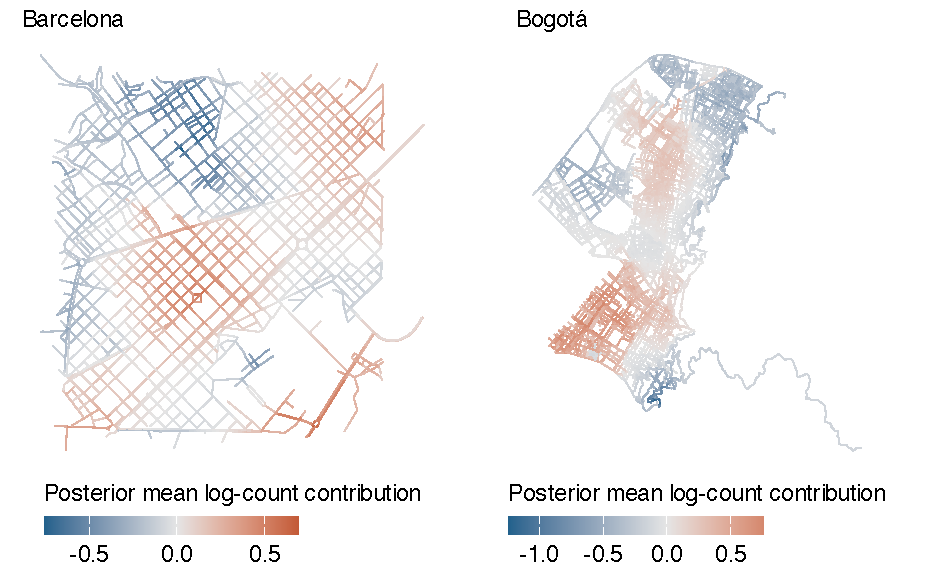
\includegraphics[width=\textwidth]{adjusted_field.pdf}
\caption{Posterior mean structured fields under recorded road attributes and estimated length. Each field combines all candidate coefficients. Colour scales are panel-specific; the maps support within-network conditional interpretation, not comparison of city-level risk.}
\label{fig:field}\end{figure}

\FloatBarrier
\subsection{Predictive contribution and comparator limitations}
The mixture and dense spectral models have almost identical pointwise scores in the matched U and C experiments (Table~\ref{tab:prediction}). Thus, allocation to spike and slab changes the description of component evidence without producing a large advantage over dense regularization on this candidate set. Introducing recorded attributes improves mixture-model ELPD by 36.6 (SE 14.2) in Barcelona and 404.7 (33.8) in Bogot\'a. The direction is consistent across all four model families, although BYM2-type estimates carry sampling warnings.

In the matched L comparison, the mixture spectral model improves on the nonspatial model by 18.1 (SE 7.2) in Barcelona and 95.4 (15.1) in Bogot\'a. This remains compatible with weak slab allocation: the spike is continuous, and the whole posterior field enters prediction. Absence of a membership probability above 0.5 is therefore not a test that all residual spatial information is absent. The Bogot\'a L mixture fit has one influential PSIS observation, with maximum Pareto $k=0.743$, so its predictive gain remains exploratory.

BYM2-type models attain the highest reported scores among the fixed-length specifications. However, all four fail the operational joint sampling criterion after their longer reruns because minimum chain E-BFMI lies between 0.191 and 0.277. Barcelona U also has maximum $\widehat R=1.012$ and minimum bulk ESS 386; Bogot\'a C has minimum bulk ESS 376. There are no divergent transitions or tree-depth saturations in the retained empirical fits. These facts do not eliminate the energy-exploration warnings, and BYM2-type numerical rankings are not treated as definitive evidence of superiority. Their estimated-length versions were not run.

\begin{table}[p]\centering\small
\caption{Exploratory pointwise PSIS-LOO results for all 20 fitted specifications. Higher ELPD is better within the same city. $n_k$ counts segments exceeding the draw-dependent Pareto threshold (approximately 0.697). ``Pass'' refers to the joint sampler criterion, not distributional adequacy. All BYM2-type results are flagged. U and C impose a unit length coefficient; L estimates it.}
\label{tab:prediction}
\begin{tabular}{llrrrl}\toprule
Model & Specification & ELPD & SE & $n_k$ & Sampler\\\midrule
\textit{Barcelona} & & & & & \\
NB & U & -3998.2 & 79.8 & 0 & Pass \\
NB & C & -3931.1 & 81.2 & 0 & Pass \\
NB & L & -3854.3 & 70.7 & 0 & Pass \\
Dense spectral & U & -3949.2 & 78.8 & 0 & Pass \\
Dense spectral & C & -3912.5 & 79.4 & 1 & Pass \\
Mixture spectral & U & -3948.9 & 78.7 & 0 & Pass \\
Mixture spectral & C & -3912.4 & 79.6 & 1 & Pass \\
Mixture spectral & L & -3836.1 & 70.0 & 0 & Pass \\
Spectral BYM2 & U & -3836.7 & 72.5 & 0 & Flagged \\
Spectral BYM2 & C & -3797.1 & 72.3 & 0 & Flagged \\
\addlinespace
\textit{Bogotá} & & & & & \\
NB & U & -20271.9 & 154.8 & 0 & Pass \\
NB & C & -19831.6 & 152.5 & 0 & Pass \\
NB & L & -19579.3 & 141.0 & 0 & Pass \\
Dense spectral & U & -20155.6 & 153.8 & 1 & Pass \\
Dense spectral & C & -19750.0 & 153.1 & 1 & Pass \\
Mixture spectral & U & -20153.9 & 153.7 & 1 & Pass \\
Mixture spectral & C & -19749.2 & 153.0 & 2 & Pass \\
Mixture spectral & L & -19483.9 & 141.3 & 1 & Pass \\
Spectral BYM2 & U & -19848.7 & 141.9 & 0 & Flagged \\
Spectral BYM2 & C & -19421.7 & 141.0 & 0 & Flagged \\
\addlinespace
\bottomrule
\end{tabular}\end{table}

\FloatBarrier
\subsection{Predictive adequacy beyond a score}
Estimating length materially improves calibration of replicated summaries. For Barcelona's mixture L model, the observed mean is 1.470 and the median replicated mean is 1.443, with a 90\% reference interval 1.324--1.567. Observed variance 7.58 is compared with a median replicated variance of 7.89 (6.30--10.68). The observed zero fraction, 0.540, lies within the replicated interval 0.513--0.558. The observed maximum of 26 is at the lower boundary of its replicated interval, indicating remaining upper-tail sensitivity.

In Bogot\'a, the mixture L model reproduces the mean and upper-count summaries more closely than the fixed-length specification. Observed mean 13.99 is compared with median replicated mean 13.87 (13.10--14.85), and observed 99th percentile 146.22 with median replicated value 146 (131.21--164.23). However, the observed zero fraction is 0.283, above the replicated interval 0.237--0.260. The conditional model still underrepresents zeros. This discrepancy motivates examination of unrecorded exposure, covariate coverage, segmentation and alternative observation models; a raw zero proportion alone would not have established that need.

Residual graph checks also qualify the spectral interpretation. Under C, median residual Moran's $I$ for the mixture model is approximately $-0.054$ in Barcelona and $0.064$ in Bogot\'a, outside the corresponding replicated reference ranges. The leading positively associated candidate patterns do not guarantee removal of dependence at all graph frequencies. Sampling success and improved pointwise scores consequently do not establish full distributional or spatial adequacy. Checks for the L fits are summarized in the supplementary material; complete numerical diagnostics belong in the computational archive.

\section{Discussion}
\subsection{What is learned from the spectral representation?}
The useful inferential object is a conditional network-supported field together with evidence about its component allocation. A graph-derived pattern is not automatically an unexplained crash pattern: adjustment for recorded attributes and the length relationship can reduce the probability of its allocation to a wider prior component. The marked decrease in membership across specifications demonstrates why a map of selected modes should be interpreted in relation to the complete observation model.

Two distinctions are especially important for GIScience. First, source eigenvectors describe the chosen topology; signed posterior contributions describe how the count model uses their transformed columns. Topological ordering alone cannot establish a substantive crash mechanism or a physical spatial scale. Second, component allocation and predictive spatial contribution are different summaries under continuous shrinkage. The L fits retain predictive information through small coefficients even when individual membership probabilities remain modest. Reporting only a thresholded list would conceal that behaviour.

Keeping segment support and candidate columns fixed makes these changes interpretable as consequences of the statistical specification rather than changes in cartographic units. Nevertheless, road-network segmentation and boundary selection remain part of the geographical model. A new segmentation can change both counts and eigenvectors. Neither the present two-city comparison nor its fixed candidate set establishes invariance to those operations.

\subsection{Scope and limitations}
The mixture formulation provides probabilistic component summaries on an existing graph-supported basis. Its novelty is the specific combination of segment support, ordered eigenvalue-informed component scales and interpretation under attribute and length adjustment. It is not the invention of Bayesian spectral filtering, and the experiments do not compare it with modern alternatives such as regularized-horseshoe filtering \citep{donegan2020}. The transformed basis also prevents describing the method as exact RENeGe covariance reduction. Prior sensitivity, alternative candidate sizes, inclusion of degree-related Perron structure and full-rank comparisons remain necessary to assess robustness beyond the reported construction.

A harmonized simulation of the present specification remains necessary to assess operating characteristics under known truth, covariate--spatial overlap and length misspecification. The present study reports the two empirical applications and does not claim simulation-based validation of the current model.

The most consequential empirical limitations concern provenance, exposure and validation. Source-to-model reconstruction establishes computational provenance, but the preserved record units, unequal periods and original spatial assignment rules limit substantive interpretation. The Bogot\'a response weights crashes by the number of person-involvement rows, and inherited road identifiers can include counts outside the final clipped geometry. Recorded road attributes require temporal alignment. Length cannot identify traffic-adjusted risk, and its fitted elasticity may absorb unmeasured traffic, road function and segmentation effects. Pointwise PSIS-LOO does not assess transfer to a withheld connected region. Outstanding Pareto cases, BYM2-type energy warnings, zero-count discrepancies and residual graph dependence each concern a different limitation; none is resolved merely by moving a table to supplementary material.

\subsection{Implications for geographical information science}
\label{sec:gis_implications}
The transferable methodological result is a way to keep geographical representation and statistical interpretation distinct while linking them in a single model. Segment adjacency specifies the relations represented by the GIS; transformed graph-derived columns provide candidate patterns; posterior allocation and signed contributions describe how those columns enter a count model. The same graph may therefore support different posterior interpretations when attributes or the length relationship change. This is a statement about conditional inference, not evidence that one adjustment must reduce spatial structure in every setting.

The distinction between allocation and the complete field also holds beyond the two applications. Under the stated prior, the covariance limit as $\pi\to0$ is $\sigma_0^2BB^{\mathsf T}$, which is nonzero for a nonzero basis and $\sigma_0>0$. Thus, interpreting weak slab allocation as a zero spatial representation would misdescribe the formulation itself. Whether the remaining field improves prediction in another dataset must nevertheless be tested; the covariance identity alone cannot establish such a gain.

For readers implementing the method, these results imply four practical steps. First, define the observational support and reconstruct adjacency on those same units. Second, distinguish raw eigenvector maps from signed posterior contribution maps. Third, compare attribute and exposure specifications while holding a candidate basis fixed within a given network. Fourth, assess component evidence, the complete field, predictive performance and residual adequacy separately. A probability threshold for slab allocation is not a substitute for checking zero-count calibration, residual graph dependence or influential observations.

The construction can be refitted to other undirected network count problems satisfying its assumptions. This mathematical transferability does not establish robustness to geographical boundaries, road segmentation, graph frequency truncation or unmeasured exposure. A changed segmentation alters both counts and graph-derived columns. Directed or temporally changing network processes are outside the evaluated formulation, and full-rank comparisons, prior sensitivity and spatially blocked validation remain necessary to assess performance beyond the retained networks.

\section{Conclusions}
This study developed an edge-supported Bayesian spectral framework for overdispersed counts on geographical networks. Its contribution to GIScience is a model-based connection between the topology and support encoded by a geographical representation and the uncertainty attached to its use in statistical inference. The framework separates topology-derived candidate patterns, posterior allocation to a wider mixture component, and the complete geographical field used for prediction. The covariance construction and continuous-spike limiting behaviour are properties of the model on any admissible fixed graph-derived basis; they do not depend on the two named cities.

This is the sense in which the methodological contribution extends beyond the applications. A new undirected network with suitable segment counts and positive exposure can be analysed by reconstructing its graph and basis and refitting the observation model. The construction transfers, while fitted coefficients, selected component identities, elasticities and predictive rankings do not transfer without new evidence. The method does not establish invariance to a changed network representation or guarantee better prediction in a new geographical setting.

In the Barcelona and Bogot\'a applications, adjustment for recorded attributes and estimation of length elasticity reduced expected slab membership, while the full spectral field retained pointwise predictive information relative to matched nonspatial models. Estimated length elasticities near 0.59 challenged proportional accumulation with length in these prepared datasets. These are conditional findings from the two retained networks, not universal estimates for urban crash processes. Their broader interpretive value is to show why a topology-derived map, a component-membership summary and a predictive spatial contribution answer different questions.

For readers, the framework provides a reusable analysis and reporting workflow: align the latent field with the observational units, distinguish candidate patterns from estimated geographical contributions, compare observation-model assumptions on a fixed basis, and report predictive and adequacy checks alongside component evidence. Weak slab membership should not be treated as proof of absent spatial information, and a smooth spectral map should not be treated as a traffic-adjusted risk surface or an explanation of a crash mechanism.

The empirical evidence remains limited by different record units and observation periods, the preserved nearest-road and pre-clipping aggregation rules, road attributes without historical alignment, and the absence of vehicle-flow exposure. The fixed 20-component basis, omitted Perron structure, connected-component restriction and untested prior and segmentation sensitivity further limit generalization. Pointwise PSIS-LOO did not evaluate transfer to unseen regions; influential observations, BYM2-type energy warnings, residual graph dependence and underprediction of zeros in Bogot\'a qualify the reported predictive results. A harmonized simulation of the current model remains outstanding.

The general contribution is an explicit formulation and interpretation for network-supported count inference under stated assumptions. Broader empirical claims require harmonized simulations, additional networks and spatially blocked validation of the current specification.

\FloatBarrier
\section*{Data and code availability statement}
The source-record projections, frozen road geometries, source hashes, commented preprocessing and Stan code, recorded sampling settings and initializations, numerical reference outputs, and finding-by-finding reproduction instructions are accessible through a single entry point: \url{https://github.com/DannaCruz/CrashBayesian/blob/main/spectral-analysis/REPRODUCIBILITY.md}. The shared projections preserve every source row, its incident identifier, year and coordinates while excluding unused personal attributes. The executable workflow reconstructs the responses and graph inputs, fits all 20 specifications, computes assessment measures, and regenerates all four main tables, five main figures, five supplementary tables and the supplementary figure. Frozen geographic inputs are included; municipal portals serve as source attribution rather than required reproduction endpoints. The guide states the distinct counting units and spatial assignment rules.

\section*{Competing interests}
The authors declare no competing financial interests or personal relationships that could have influenced the work.

\section*{Use of generative AI}
OpenAI Codex assisted with code development, data checks, figure preparation, manuscript restructuring and language editing. Verification of the data, statistical interpretation and responsibility for the work rest with the authors.

\bibliographystyle{plainnat}
\bibliography{references}
\end{document}
